\chapter{High Performance Computing (HPC)} \label{HPC1}
\section{Introduction}
Supercomputing has developed early in the 1970s with CDC 6600, ILLIAC-IV and the generation of CRAY. The high performance computing (HPC) was born in context of scientific computing. In fact, It was a challenge to be fast and more precise when were talking about scientific computing such as simulation purposes like weather forecasting, numerical mechanics for car crash tests, financial market prediction or other various complex phenomena modelings. The HCP's development was also accompanied with new paradigm in the computer design in hardware and software levels. It takes more advantages in the concepts of parallel system and parallel program, shared and distributed memory. Thus, the high performance computers as
machines with a good balance among the following major elements \cite{Rubin}
\begin{itemize}
\item Multistaged (pipelined) functional units.
\item Multiple central processing units (CPUs) (parallel machines).
\item Multiple cores. 
\item Fast central registers.
\item Very large, fast memories.
\item Very fast communication among functional units.
\item Vector, video, or array processors.
\item Software that integrates the above effectively.
\end{itemize}

Today, with Moore's Laws, the performance of computer is continuously increasing. In 2017, the Top500\footnote{\url{https://www.top500.org}}, website ranking the list of the top 500 supercomputers, classifies the Sunway TaihuLight (a system developed by \textit{China's National Research Center of Parallel Computer Engineering \& Technology} (NRCPC)) to be the most power computer in the world. The Sunway TaihuLight has a note of 93 Petaflops in Linpack Performance, where a Petaflops is $10^{15}$ floating-point operations per second. Recently, the Atos group has launched a new generation of quantum learning machines that can reach 24 TB of memory and 16 CPU, with power of from 30 to 40 Qubits (see \ref{qlm}). These computers allows researchers, engineers and students to develop and experiment with quantum software.   
\begin{figure}[!h]
% Use "\centering" in floats (figure, table), but if you need to center
% some text (why?) use "\begin{center}...\end{center}".
\centering 
% Figure environments same as 0.8 * \textwidth please
% That does not necessarily mean the actual picture size,
% it is a guideline for the environment which could contain
% 2 or more pictures! Be consistent and follow the guidelines
% provided in your sources.

\includegraphics[width=0.6\textwidth]{images/qlm.png}
\caption{ATOS quantum learning machine}
\label{qlm} 
% if you move the label it breaks the reference numbering; 
% always have it *after* the caption.
\end{figure}
\section{HPC architecture}
Several effort has been doing in single processor performance by the ever-increasing density of transistors-the electronic switches-on integrated. The small dimension of transistors in an integrated circuit has increased the speed of this circuit. Therefore, this fact implies the increase of the heat of these transistors due to the power consumption. However, the air-cooled integrated circuits are reaching the limits of their ability to dissipate heat, in the first decade of the twenty-first century \cite{Hager2010}. 
Therefore, it is not sure to continue to increase the speed of integrated circuits. The chip's industries have another option instead to spend much money for building ever-faster, more complex, monolithic
processors. They decide to put multiple, relatively simple, complete processors on a single chip, called multicore. Each core represents a CPU. Now, Programmers have to take into account the parallel architecture to be more efficient and more faster. 
In the parallel systems, different concepts are used  : SIMD (\textit{Single Instruction, Multiple Data}), MIMD (\textit{Multiple Instruction, Multiple Data}), Shared Memory, Distributed Memory, Interconnection networks \cite{Hager2010}. 

\subsection{SIMD} \label{simb} A concept of Flynn's taxonomy, SIMD indicates the fact that multiple processing units (core) execute the same instruction on multiple data streams. Each processing unit can perform on different data elements. The figure \ref{simb} gives an example of SIMD execution on three CPU.The SIMD is used for specialized problems characterized by a high degree of regularity, such as graphics/image processing (GPUs). In addition, SIMD is used in the architecture of vector processors which enable to vectorize loop in matrix calculation (see figure \ref{vector}).  
Example of SIMD Processor Arrays and Vector Pipelines : Thinking Machines CM-2, MasPar MP-1 \& MP-2, ILLIAC IV, IBM 9000, Cray X-MP, Y-MP \& C90, Fujitsu VP, NEC SX-2, Hitachi S820, ETA10.
\begin{figure}[!h]
\centering 
  \begin{subfigure}[b]{0.4\textwidth}
    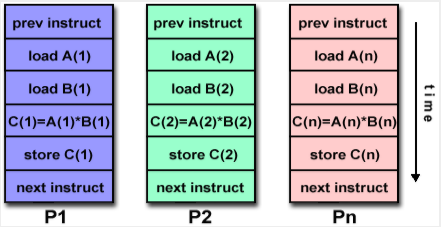
\includegraphics[width=\textwidth]{images/simd.png}
    \caption{SIMD Instruction}
    \label{simb}
  \end{subfigure}
  %
  \begin{subfigure}[b]{0.4\textwidth}
    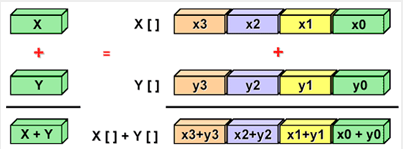
\includegraphics[width=\textwidth]{images/vectorization.png}
    \caption{SIMD Vectorization}
    \label{vector}
  \end{subfigure}
  \caption{Single Instruction, Multiple Data (SIMD)}
\end{figure}

\subsection{MIMD} As the name suggests, MIMD or multiple instruction streams on multiple processors (cores) operate on different data items concurrently. MIMD systems typically consist of a collection of fully independent processing units or cores, each of which has its own control and logical unit. The execution process can be synchronous or asynchronous, deterministic or non-deterministic . The MIMD architecture is found in most current supercomputers, networked parallel computer clusters and "grids", multi-processor SMP computers, multi-core PCs. The figure  shows an example of MIMD execution.  
\begin{figure}[!h]
\centering 
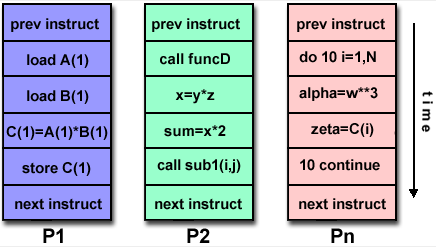
\includegraphics[width=0.6\textwidth]{images/mimd.png}
\caption{Multiple Instruction, Multiple Data (MIMD)}
\label{sim1} 
% if you move the label it breaks the reference numbering; 
% always have it *after* the caption.
\end{figure}

\subsection{Shared Memory} A shared-memory system is a collection of autonomous processors (cores) connected to memory via an interconnection network, and processors share physical address of memory \cite{Hager2010}. There are two different memory access in shared-memory system: Uniform Memory Access (UMA) and cache-coherent Non-uniform Memory Access (ccNUMA). 

The UMA can be considered a 'flat' memory model, because latency and an bandwith are the same for all cpu and all memory location. Sometimes called Symmetric Multiprocessor (SMP), UMA system  enables to have equal access and equal time to memory. The general problem of UMA machines is that bandwidth bottlenecks are bound to occur when the number of sockets is larger than a certain limit. The figure \ref{uma} show a representation of UMA architecture. 
In ccNUMA, memory is physically distributed but logically shared (see figure \ref{numa}). This architecture seems to be distrubuted-memory system, but network logic makes the aggregated memory of the whole system appear as
one single address space. This simplify the memory access without resorting to a network of any kind. The locality domain (LD), set of processor cores connected locally to memory,can be considered as a UMA "building block". The ccNUMA principle gives scalable bandwidth for very large processor counts. It can be inexpensive small for two- or four-socket nodes frequently used for HPC clustering \cite{Hager2010}.

The LD can be, sometimes, an obstacle for high performance software on ccNUMA. The second problem is potential
contention if two processors from different locality domains access memory in the same locality domain, fighting for memory bandwidth. Both problems can be solved by carefully observing the data access patterns of an application and restricting data access of each processor to its own locality domain \cite{Hager2010}.
\begin{figure}[!h]
\centering 
  \begin{subfigure}[b]{0.4\textwidth}
    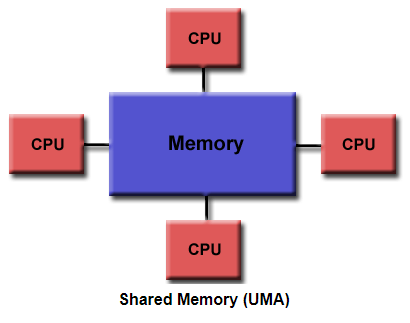
\includegraphics[width=\textwidth]{images/uma.png}
    \caption{Shared-Memory (UMA)}
    \label{uma}
  \end{subfigure}
  %
  \begin{subfigure}[b]{0.4\textwidth}
    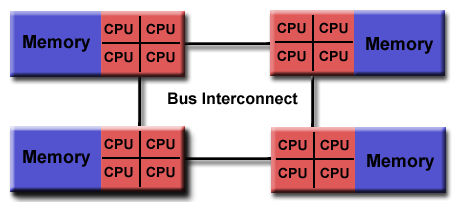
\includegraphics[width=\textwidth]{images/numa.png}
    \caption{Shared-Memory (NUMA)}
    \label{numa}
  \end{subfigure}
\end{figure}
\subsection{Distributed Memory}
In the distributed-memory system, each processor is connected to exclusive local memory and network communication connect also inter-processor memory (see \ref{dmemory}). The memory is scalable with the number of processor and we are a rapid access of each processor with its own memory. However, the programmer must explicitly define how to access data when a processor need it in another one. Besides, the programmer is also responsible to handle the synchronization task \cite{Hager2010}.
\begin{figure}[!h]
\centering 
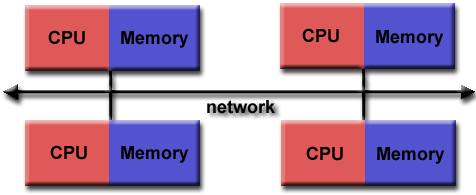
\includegraphics[width=0.4\textwidth]{images/d-memory.png}
\caption{Distributed Memory}
\label{dmemory} 
\end{figure}

According to \cite{Hager2010}, there are actually no distributed-memory systems any more that implement such a layout where we HPC clustering. Most of parallel systems couple at same time shared and distributed systems (Hybrid Systems) i.e. there are shared-memory building blocks connected via a fast network. This Hybrid Distributed-Shared Memory make the system to take advantages of the two architectures and the increase of the scalability. The figure \ref{hybrid} shows an Hybrid architecture with CPU and GPU (\textit{Graphical Processing Unit}) cores.
\begin{figure}[!h]
\centering 
  \begin{subfigure}[b]{0.4\textwidth}
    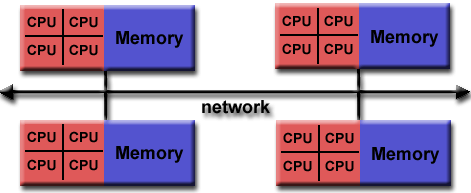
\includegraphics[width=\textwidth]{images/hybrid1.png}
  \end{subfigure}
  %
  \begin{subfigure}[b]{0.4\textwidth}
    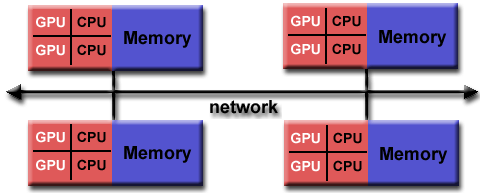
\includegraphics[width=\textwidth]{images/hybrid2.png}   
  \end{subfigure} 
   \caption{Hybrid System with CPU/GPU cores}
   \label{hybrid}
\end{figure}
\subsection{Interconnection networks}
In HPC domain, the interconnect plays a crucial role for latency and bandwidth performance of both distributed- and shared-memory systems.

\begin{figure}[!h]
\centering 
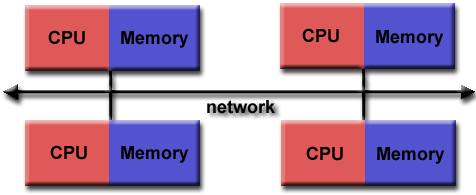
\includegraphics[width=0.4\textwidth]{images/d-memory.png}
\caption{Interconnected Networks with different topologies}
\label{dmemory} 
\end{figure}


\section{Parallel Programming} \label{scalability}
The parallel programming paradigm has been invented in the purpose of reducing the complexity of computation of certain problem. This implies have to be divided  in multiple task that are working simultaneously in different processors unit. Early in 1960's, companies (like Intel, CRAY, IBM and others) and researchers had been working together to define the design of the supercomputer. Amdahl, research at Intel, was the first theoretical approach of speedup and efficiency of the computer system. Amdahl's law has improved the performance of the parallel computers. We witnessed another approach to compute the speedup and efficiency defined by Gustafson. All this approach measure the performance of the system in term of scalability. 

\subsection{Scalability}
Whatever parallelization scheme is chosen, this perfect picture will most probably not hold in reality. The performance of parallel programs depends on multiple features such as algorithmic limitations, bottlenecks (see Figure \ref{bottlenecks}), load balancing (e Figure \ref{loadbalancing}), communication processes (e Figure \ref{communication}) startup overhead etc. All this effects imply the limit of the speedup in other term the scalability. According to [], a parallel program
is \textit{scalable} if there is a rate at which the problem size can be increased so that as the
number of processes/threads is increased, the efficiency remains constant. In the context parallel system,  scalabality can be seen in two ways: \textit{'strong'} scalability and the \textit{'weak'} scalability. We say a program is \textit{strongly} scalable, if the problem size can remain fixed, and it's \textit{weakly} scalable if the problem size needs to be increased at the same rate as the number of processes/threads.  

\begin{figure}[!h]
\centering 
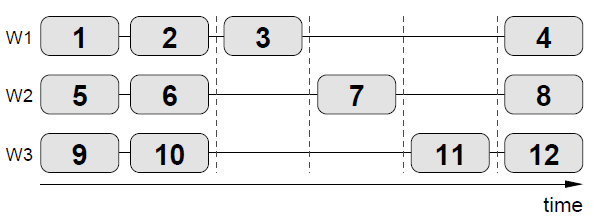
\includegraphics[width=0.4\textwidth]{images/bottlenecks.png}
\caption{Parallelization with a bottleneck. Tasks 3, 7 and 11 cannot overlap with anything else across the dashed "barriers."}
\label{bottlenecks} 
\end{figure}
\begin{figure}[!h]
\centering 
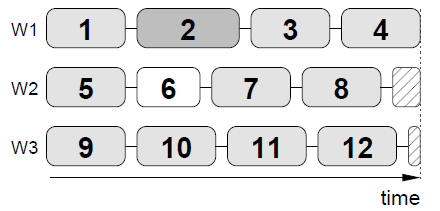
\includegraphics[width=0.4\textwidth]{images/loadbalancing.png}
\caption{Some tasks executed by different workers at different speeds lead to load imbalance. Hatched regions indicate unused resources.}
\label{loadbalancing} 
\end{figure}
\begin{figure}[!h]
\centering 
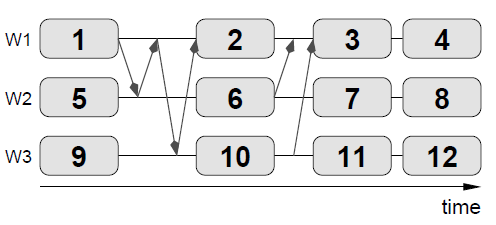
\includegraphics[width=0.4\textwidth]{images/communication.png}
\caption{Communication processes (arrows represent messages) limit scalability if they cannot be overlapped with each other or with calculation.}
\label{communication} 
\end{figure}

\subsection{Speedup} 
Finding parallelism is not only a common problem in computing but also in many other areas like manufacturing, traffic flow and even business processes. In a very simplistic view, all execution units (workers, assembly lines, waiting queues, CPUs, ...) execute their assigned work in exactly the same amount of time. \newline
Using parallel hardware, when we run a program with \textit{p} cores, one thread or process for each core, then the parallel program will run p times faster than the serial program. When the parallel time is noticed by $T_{parallel}$ and the serial time by $T_{serial}$ then the $T_{parallel}$ will now ideally take only $T_{serial}/p$. We call the program has \textbf{linear speedup} (book parallel-program). \newline
Formally, the \textit{speedup} of a parallel program can be defined to be:
\begin{equation}
S = \frac{T_{serial}}{T_{parallel}}
\end{equation} 
Moreover, the \textbf{efficiency} of parallel program is defined to be the rapport of the speedup and the number of process.
\begin{equation}
\frac{S}{p} = \frac{\frac{T_{serial}}{T_{parallel}}}{p} = \frac{T_{serial}}{T_{parallel}.p}
\end{equation} 

For a fixed problem solving with a single-worker (serial), the runtime is given by:
\begin{equation}
T_{f}^{s} = s + p 
\end{equation}
where s is the serial(nonparallelizable) part and p is the perfectly parallelizable fraction. \newline
Solving the same problem on N workers (parallel) will require a runtime of
\begin{equation}
T_{f}^{p} = s + \frac{p}{N}
\end{equation}
This is called \textit{strong scaling} because the amount of work stays constant no matter how many workers are used. Here the goal of parallelization is minimization of time to solution for a given problem.

In the context of \textit{weak scalability}, we assume that the serial runtime for the same problem is.
\begin{equation}
T_{f}^{s} = s + pN^{\alpha} 
\end{equation}
Consequently, the parallel runtime is
\begin{equation}
T_{f}^{p} = s + pN^{\alpha - 1} 
\end{equation}
\subsection{Amdahl's Law}
The application \textit{speedup} can be defined as the quotient of parallel and serial performance for fixed problem size. Here we define "performance" as "work over time," unless otherwise noted. Serial performance for fixed problem size (work) $s+ p$ is thus.
\begin{equation}
P_{f}^{s} =  \frac{s+p}{T_{f}^{s}}  = 1
\end{equation}
as expected. Parallel performance is in this case
\begin{equation}
P_{f}^{p} =  \frac{s+p}{T_{f}^{p}(N)}  = \frac{1}{s + \frac{1-s}{N}}
\end{equation}
and application \textit{speedup} ("scalability") is
\begin{equation}
S_{f} =  \frac{P_{f}^{p}}{P_{f}^{s}}  = \frac{1}{s + \frac{1-s}{N}}
\end{equation}
This is called \textit{Amdahl's law}, which was first conceived by Gene Amdahl in 1967. It limits application speedup for $N \rightarrow N $ to $1/s$.
Let's consider only the parallelizable part of the calculation (for which there may be sound reasons at first sight), we get the serial performance :
\begin{equation}
P_{f}^{sp} =  \frac{p}{T_{f}^{s}}  = p
\end{equation} 
since $T_{f}^{s} = s+p = 1$. We derive the parallel performance to be.
\begin{equation}
P_{f}^{pp} =  \frac{p}{T_{f}^{p}}  = \frac{1-s}{s + \frac{1-s}{N}}
\end{equation}
Therefore, we find the \textit{Amdahl's law}:
\begin{equation}
S_{f} =  \frac{P_{f}^{pp}}{P_{f}^{sp}} = \frac{1}{s + \frac{1-s}{N}}
\end{equation}
Although scalability does not change with this different notion of "work," performance does, and is a factor of p smaller.
If we consider the weak scaling, the serial performance can be defined to be :
\begin{equation}
P_{v}^{s} =  \frac{s+p}{T_{f}^{s}}  = 1
\end{equation}

and the parallel performance is .
\begin{equation} \label{eq1}
P_{f}^{p} =  \frac{s+pN^{\alpha}}{T_{f}^{p}(N)}  = \frac{s+(1-p)N^{\alpha}}{s+pN^{\alpha -1}} = S_v
\end{equation}
again identical to application speedup. In the special case $\alpha = 0$ (strong scaling) we recover Amdahl's Law. With $0 <a < 1$, we get for large CPU counts.
\begin{equation}
S_v = \longrightarrow^{N \gg 1} \frac{s+(1-p)N^{\alpha}}{s} = 1 + \frac{p}{s} N^{\alpha}
\end{equation}
As a result, weak scaling allows us to cross the Amdahl Barrier and get unlimited performance, even for small $\alpha$. In the ideal case $\alpha = $, the equation \ref{eq1} is simplified to
\begin{equation}
S_v(\alpha = 1)= s + (1-s)N
\end{equation}
This is called \textit{Gustafson's Law}. The speedup is linear. Therefore, Gustafson's law addresses the lack of Amdahl's law, which is based on the assumption of a fixed problem size. Generally, in scientific simulations, researchers tend to increase the size of the problem to know the improvement of the resources. Hence,Gustafson's law allow to exploit the computing power that becomes available as the resources improve.
 
The parallel efficiency is also defined to be the rapport between performance on N CPUs $P_N$ and the product of the N and the performance on one CPU $P_1$.
\begin{equation}
\epsilon = \frac{P_N}{P_1} = \frac{Speedup}{N}
\end{equation}
\subsection{Shared Memory Parallel Programming: OpenMP} \label{openMP}
As we said above, the shared-memory and the multicores systems architectures allow to get more performance with \textit{"multiprocessing"} or \textit{multi-threading} programming paradigm. All cores work concurrently in different parallel regions of the memory to give at the end the result of the instruction. In Shared-Memory programming, \textbf{OpenMP} \footnote{http://www.OpenMP.org} (\textit{Open Multi-Processing}) like Pthreads and other tools have been used to exploit the multicores resources. We give here a brief description of the library OpenMP which is used in DSFDM/FFWI code.

The OpenMP is library created in 1997 and it is used in C, C++, and Fortran languages to support the multiprocessing programming paradigm in parallel systems. OpenMP is a set of compiler directives that a non-OpenMP-capable compiler would just regard as comments and ignore. Hence, a well-written parallel OpenMP program is also a valid serial program. The central entity in an OpenMP program is not a process but a thread. Threads are also called "lightweight processes" because several of them can share
a common address space and mutually access data. Each thread can, by means of its local stack pointer, also have "private"
variables, but since all data is accessible via the common address space, it is only a matter of taking the address of an item to make it accessible to all other threads as well. However, the OpenMP standard actually forbids making a private object available to other threads via its address.
\begin{figure}[!h]
\centering 
\includegraphics[height=8cm,width=5cm]{images/OpenMP.png}
\caption{Model for OpenMP thread operations}
\label{OpenMP} 
\end{figure}

The figure \ref{OpenMP} shows in details how OpenMP thread works. In OpenMP program, a single thread, the master thread, runs immediately after startup. Truly parallel execution happens inside parallel regions, of which an arbitrary number can exist in a program. Between two parallel regions, no thread except the master thread executes any code. This is also called the "fork-join model". Inside a parallel region, a team of threads executes instruction streams concurrently. The number of threads in a team may vary among parallel regions. 

We give above, as example, a simple OpenMP program in Fortran which enables the numerical integration of the following function:
\begin{equation}\label{pi}
\pi = \int_{0}^{1}dx \frac{4}{1+x^2}
\end{equation}

\begin{lstlisting}[language=Fortran, caption= Listing code of  numerical integration of \ref{pi}]
double precision :: pi,w,sum,x
integer :: i,N=1000000

pi = 0.d0
w = 1.d0/N
sum = 0.d0
!$OMP PARALLEL PRIVATE(x) FIRSTPRIVATE(sum)
!$OMP DO
do i=1,n
 x = w*(i-0.5d0)
 sum = sum + 4.d0/(1.d0+x*x)
 enddo
 !$OMP END DO
 !$OMP CRITICAL
  pi= pi + w*sum
 !$OMP END CRITICAL
 !$OMP END PARALLEL
\end{lstlisting}

In this simple code, every thread executes all code enclosed in the parallel region  and OpenMP library routines are used to obtain thread identifiers and total number of threads. There exists other compiler directives that are available on the official documentation [http://www.OpenMP.org].

\subsection{Distributed Memory Parallel Programming: MPI} \label{MPI}
The second programming model is the \textit{Message Passing} which is dedicated for distributed memory system. The \textit{Message Passing Interface} (\textbf{MPI}) was designed early 1990s to facilitate the communication between processes. The MPI library was coming after many standardization efforts between industrials and scientific community, to allow parallel program to be easily portable between platforms. It is regarded as a necessary ingredient in any HPC system installation, and numerous types of interconnect are supported \cite{Hager2010}. 

We can remember that MPI is just a standard but its implementation is available under different distributions such as \textit{MVAPICH}, \textit{Open MPI}, \textit{Intel MPI}, \textit{IBM BG/Q MPI} and \textit{IBM Spectrum MPI}. The main implementations are written in language like Fortran, C or C++. The DSFDM/FFWI code was compiled with \textit{Intel MPI}. 

This simple example of "Hello World" give an overview of a parallel program using MPI \cite{Hager2010}. 
\begin{lstlisting}[language=Fortran, , caption= Listing code of "Hello World" in parallel]
 program helloWorld 

 use MPI

 integer :: rank, size, ierror

 call MPI_Init(ierror)
 call MPI_Comm_size(MPI_COMM_WORLD, size, ierror)
 call MPI_Comm_rank(MPI_COMM_WORLD, rank, ierror)

 write(*,*) 'Hello World, I am ',rank,' of ',size

 call MPI_Finalize(ierror)
\end{lstlisting}

In this example, the call of \verb|MPI_Init()| initializes the parallel environment. Upon initialization, MPI sets up the so-called world communicator, which is called \verb|MPI_COMM_WORLD|. A communicator defines a group of MPI processes that can be referred to by a communicator handle. The \verb|MPI_COMM_WORLD| handle describes all processes that have been started as part of the parallel program. If required, other communicators can be defined as subsets of \verb|MPI_COMM_WORLD|. Nearly all MPI calls require a communicator as an argument. The calls to \verb|MPI_Comm_size()| and \verb|MPI_Comm_rank()| in lines 8 and 9
serve to determine the number of processes (size) in the parallel program and the unique identifier (\verb|rank|) of the calling process, respectively. Note that the C bindings require output arguments (like rank and size above) to be specified as
pointers. The ranks in a communicator, in this case \verb|MPI_COMM_WORLD|, are consecutive, starting from zero. In line 13, the parallel program is shut down by a call to \verb|MPI_Finalize()|. Note that no MPI process except rank 0 is guaranteed to
execute any code beyond \verb|MPI_Finalize()|.

The table \ref{MPItable} shows some point to point and collective communication routines for MPI (Fortran subroutines).
\begin{table}[!h]
\centering
\begin{tabularx}{\linewidth}{|X|X|}
\hline
\textbf{subroutine} & \textbf{Description} \\
\hline
\hline
\verb|MPI_SEND()| & Basic blocking send operation. Routine returns only after the application buffer in the sending task is free for reuse. \\
\hline
\verb|MPI_RECV()| & Receive a message and block until the requested data is available in the application buffer in the receiving task. \\
\hline
\verb|MPI_SSEND()| & Synchronous blocking send: Send a message and block until the application buffer in the sending task is free for reuse and the destination process has started to receive the message. \\
\hline
\verb|MPI_SENDRECV()| & Send a message and post a receive before blocking. Will block until the sending application buffer is free for reuse and until the receiving application buffer contains the received message. \\
\hline
\verb|MPI_WAIT()| & \verb|MPI_Wait| blocks until a specified non-blocking send or receive operation has completed. \\
\hline
\verb|MPI_Probe()| & Performs a blocking test for a message. The "wildcards" \verb|MPI_ANY_SOURCE| and \verb|MPI_ANY_TAG| may be used to test for a message from any source or with any tag. \\
\hline
\verb|MPI_GET_COUNT()| & Returns the source, tag and number of elements of datatype received.\\
\hline
\verb|MPI_BARRIER ()| & Synchronization operation. Creates a barrier synchronization in a group. Each task, when reaching the \verb|MPI_Barrier| call, blocks until all tasks in the group reach the same \verb|MPI_Barrier| call. \\
\hline
\verb|MPI_BCAST()| & Data movement operation. Broadcasts (sends) a message from the process with rank "root" to all other processes in the group.\\
\hline
\verb|MPI_SCATTER()| & Collective computation operation. Applies a reduction operation on all tasks in the group and places the result in one task. \\
\hline
\verb|MPI_ALLREDUCE()| & Collective computation operation + data movement. Applies a reduction operation and places the result in all tasks in the group. \\
\hline
\verb|MPI_REDUCE_SCATTER()| & Collective computation operation + data movement. First does an element-wise reduction on a vector across all tasks in the group. \\
\hline
\verb|MPI_ALLTOALL()| & Data movement operation. Each task in a group performs a scatter operation, sending a distinct message to all the tasks in the group in order by index.\\
\hline
\end{tabularx}
\caption{\label{MPItable} MPI communication routines}
\end{table}

\section{Optimization Techniques in HPC} \label{optimization}
The principal objective that encouraged the use of HPC comes from a real need to improve the performance of scientific and industrial problems which require a great spatial and temporal complexity. In this optic, HPC applications need to optimize their communications and synchronizations to deliver high performance. Although the advanced of modern CPU, the increasing of memory storage and the improvement of interconnection networks, optimization is a difficult and often tedious process, it is usually more cost-effective than investing in additional system resources. In the context of parallel system, the optimization is composed of set of elements that must be taken into account together to do the program more efficient. These elements includes compilers directives, multi-threaded optimization, SIMD vectorization, placement of MPI processes, optimization libraries, code profiling.

\subsection{Compiler Optimization}
Compilers are the basic tools applied to HPC applications to get good performance from the target hardware. Usually, several compilers are available for each architecture. The most important languages for High Performance Computing are FORTRAN, C, and C++ because they are the ones used by the vast majority of codes. GNU Compiler Collection (GCC) and Intel are the most used compiler in HPC. Here, we gives briefly some important compiler directives to optimize the HPC code.
\begin{itemize}
\item \textbf{GNU Compiler (GCC)}
The GNU compiler tool chain contains front ends for C, C++, Objective-C, FORTRAN, Java, Ada, and Go, as well as libraries for these languages. These compilers are 100\% free software and can be used on any system independently of the type of hardware. It is the default compiler for the Linux operating system and is shipped with it []. The GCC/GFortran compiler has to be configured and compiled on a specific target system, so it may not support some features and compiler technologies depending on the configure arguments. The table \ref{GCC} shows a list of gnu optimizer options. Flags are obtained with gcc/gfortarn -Q --help=optimizers (GNU Compiler documentation\footnote{\url{https://gcc.gnu.org/onlinedocs/}}).
\begin{table}[!h]
\centering
\begin{tabularx}{\linewidth}{|X|X|}
\hline
\textbf{GCC compiler option} & \textbf{Explanation} \\
\hline
\hline
-march= & Generate code for given CPU for example "corei7-avx" Sandy Bridge CPU and use autovectorization AVX \\
\hline
-mtune= & Schedule code for given CPU \\
\hline
-O0 & Reduce compilation time and keep execution in the same order as the source line listing so that debugging produces the expected results. This is the default. \\
\hline
-O or -O1  & The first optimization level. Optimizing compilation takes more time and a lot more memory for a large function.

With -O/-O1, the compiler tries to reduce code size and execution time, avoiding any optimizations that take would significantly increase compilation time. \\
\hline
-O2 &  The second optimization level. GCC performs nearly all supported optimizations that do not involve a space-speed tradeoff. As compared to -O, this option increases both compilation time and the performance of the generated code. \\
\hline
-Os & Optimize for size. -Os enables all -O2 optimizations that do not typically increase code size. It also performs further optimizations designed to reduce code size. \\
\hline
-O3 & The third optimization level. -O3 turns on all optimizations specified by -O2. \\
\hline
\end{tabularx}
\caption{\label{GCC} GNU Compiler options}
\end{table} 

\item \textbf{Intel Compiler}
The Intel compiler suite is traditionally the most efficient compiler for the Intel CPU as it is designed by Intel. The latest features of the Intel processors Intel Xeon are implemented in the Intel Intel® Parallel Studio XE []. It includes a FORTRAN, C, and C++ compiler, an MKL library, VTune and Intel Advisor profiler, and other components (Cilk, IPP, TBB, ). The following compiler directives in \ref{Intel} enable the general optimization option in Intel CPU using Intel Compiler (see Intel Compiler documentation\footnote{\cite{https://software.intel.com/en-us/intel-cplusplus-compiler-17.0-user-and-reference-guide}} ).

\begin{table}[!h]
\centering
\begin{tabularx}{\linewidth}{|X|X|}
\hline
\textbf{Intel compiler option} & \textbf{Explanation} \\
\hline
\hline
-O0 & No optimization. Used during the early stages of application
development and debugging. Use a higher setting when the
application is working correctly \\
\hline 
-Os or -O1 & Optimize for size. Omits optimizations that tend to increase object
size. Creates the smallest optimized code in most cases.
These options may be useful in large server/database applications
where memory paging due to larger code size is an issue. \\
\hline 
-O2 & Maximize speed. Default setting. Enables many optimizations, including
vectorization. Creates faster code than -O1 in most cases. \\
\hline 
-O3  & Enables -O2 optimizations plus more aggressive loop and
memory-access optimizations, such as scalar replacement, loop
unrolling, code replication to eliminate branches, loop blocking to
allow more efficient use of cache and additional data prefetching.

The -O3 option is particularly recommended for applications
that have loops that do many floating-point calculations or process
large data sets. These aggressive optimizations may occasionally
slow down other types of applications compared to -O2. \\ 
\hline 
-qOpenMP & Causes multi-threaded code to be generated when OpenMP
directives are present. For Fortran only, makes local arrays automatic
and may require an increased stack size. See http://www.OpenMP.org
for the OpenMP API specification. \\
\hline 
-parallel & The auto-parallelizer detects simply structured loops that may be
safely executed in parallel, including loops implied by Intel$^{\mbox{\scriptsize{\textregistered}}}$ Cilk\texttrademark  Plus
array notation, and automatically generates multi-threaded code for
these loops. \\
\hline

-mkl=\textit{name} & Requests that the Intel$^{\mbox{\scriptsize{\textregistered}}}$ Math Kernel Library (Intel$^{\mbox{\scriptsize{\textregistered}}}$ MKL) be linked.
Off by default. Possible values of name are:

parallel Links the threaded part of Intel MKL (default)

sequential Links the non-threaded part of Intel MKL

cluster Links the cluster and sequential parts of Intel MKL \\

\hline
\end{tabularx}
\caption{\label{Intel} Intel Compiler options}
\end{table}
\end{itemize}
\subsection{Vectorization}
The HPC program can get more performance by using the vectorization capability of modern CPU. Vectorization allows you to execute a single instruction on multiple data (SIMD) objects in parallel within a single CPU core (see section \ref{simb}). This is different from task parallelism using MPI, OpenMP or other parallel libraries where additional cores or nodes are added to take care of data belonging to separate tasks placed on different cores or nodes. The industry of microprocessor has developed SIMD vectorization in the architecture of the modern CPU. AVX (Advanced Vector Extensions) and SSE (Streaming SIMD Extensions) are two vector instructions available in most supercomputers. AVX were introduced by Intel with the\textit{ Sandy Bridge} processor shipping in 2011 and later that year by AMD with the Bulldozer processor.  AVX instructions simultaneously operate on 8 pairs of single precision (4 bytes) operands or 4 pairs of double precision (8 bytes) operands, etc. This can speed up a vectorizable loop by up to 8 times in case of single precision (4 bytes), or 4 times in case of double precision (8 bytes), etc. There exists an extension AVX 2 which expands most integer commands to 256 bits and introduces fused multiply-accumulate (FMA) operations. The SSE is a SIMD instruction set extension to the x86 architecture, designed by Intel and introduced in 1999 in their Pentium III. It use 128-bit registers to operate simultaneously on two 64-bit (8-byte) double precision numbers, four 32-bit (4-byte) floating point numbers, two 64-bit integers, four 32-bit integers, eight 16-bit short integers or sixteen 8-bit bytes. 

The vectorization can be done by calling OpenMP directives or it is performed automatically after an using appropriate compiler flags. The following example vectorizes a loop .
\begin{lstlisting}[language=Fortran, , caption= Listing code of loop vectorization]
subroutine sub(a,b,n,k)
integer n, k
real a(n), b(n)
integer i

!$omp simd vectorlength(8)
do i=k+1,n

   a(i) = 0.5 * (a(i-k) + b(i-k))

end do

end
\end{lstlisting}

We can also use the auto-vectorization with the directive "-O3 SSE3", "-O3 -xAVX" or "-O3 -xCORE-AVX2".  
\subsection{Threading/Multi-threading}
Exploiting the multithreading techniques can increase considerably the performance of HPC code. As we said above, the threading model for HPC is handled by OpenMP or Pthread. In the thread level parallelism (TLP), the parallel code will get performance where the number of threads is increased and threads are instantiated and executed independently. However, multi-threading keeps CPU busy by engaging multiple threads. By using OpenMP threads, we study in section the scalability of DSFDM/FFWI code in multi-threading level. 

The \textit{Hyper-threading} and \textit{Affinity} are features of performance in many Intel$^{\mbox{\scriptsize{\textregistered}}}$ CPU (Intel$^{\mbox{\scriptsize{\textregistered}}}$ Core\texttrademark vPro   \texttrademark processors, the Intel$^{\mbox{\scriptsize{\textregistered}}}$ Core\texttrademark processor family, the Intel$^{\mbox{\scriptsize{\textregistered}}}$ Core\texttrademark M processor family, and the Intel $^{\mbox{\scriptsize{\textregistered}}}$ Xeon$^{\mbox{\scriptsize{\textregistered}}}$ processor family). \textit{Hyper-threading} is Intel's proprietary simultaneous multithreading (SMT) implementation used to improve parallelization of computations performed on x86 microprocessors. Instructions from more than one thread can be executing in any pipeline stage at a time. \textit{Thread Affinity} is the ability to bind threads to physical processing units. Thread affinity restricts execution of certain threads (virtual execution units) to a subset of the physical processing units in a multiprocessor computer. Depending upon the topology of the machine, thread affinity can have a dramatic effect on the execution speed of a program. the \verb|KMP_AFFINITY| environment variable controls the affinity interface in OpenMP. There are three ways to manage the type of affinity: \textit{none}(default), \textit{compact}, \textit{scatter}. The figures [\ref{scatter}, \ref{compact}] show the difference between \textit{compact} and \textit{scatter}.

\begin{figure}[!h]
\centering 
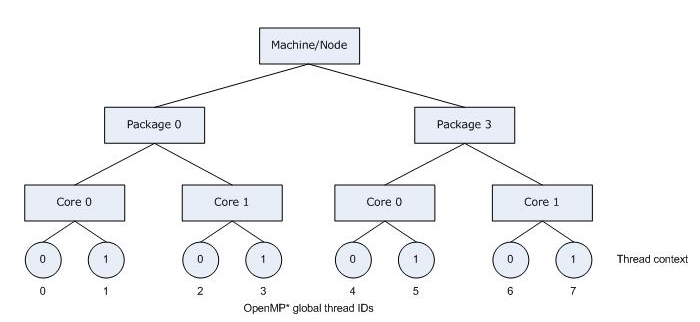
\includegraphics[height=6cm,width=12cm]{images/compact.png}
    \caption{Compact affinity: $KMP\_AFFINITY=granularity=fine,compact$.}
\label{compact} 
\end{figure}  

\begin{figure}[!h]
\centering 
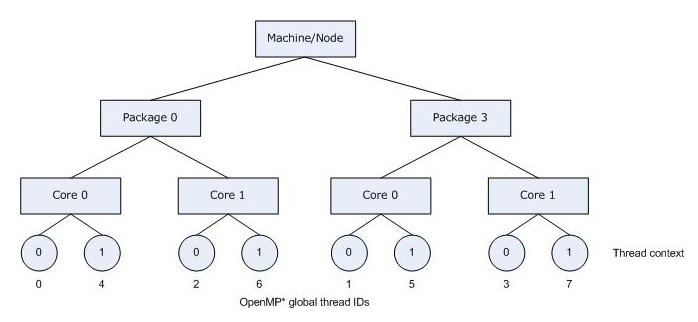
\includegraphics[height=6cm,width=12cm]{images/scatter.png} 
    \caption{Scatter affinity: $KMP\_AFFINITY=granularity=fine,scatter$.}  
\label{scatter} 
\end{figure}  
\subsection{MPI processes} 
MPI, \textit{Massage Passing Interface}, dedicated for parallel distributed system have great impact for code optimization in HPC environment. For more details see \ref{MPI}. The study of scalability, in section \ref{dsfdm}, gives more details of the performance of DSFDM/FFWI. 
\subsection{Code Profiling} \label{profiling}
Code Profiling helps in identifying algorithmic bottlenecks (hotspots), and also communication overheads in case of distributed code. Most of the execution time can be spent in the function which is repeatedly calling other slower functions or there can be slower pieces in the code. Several tools are available for profiling. \textit{Gprof} is most frequently used in the HPC community. There are advanced profilers used in the context of this \textit{Advisor} and \textit{VTune} Amplifier from Intel$^{\mbox{\scriptsize{\textregistered}}}$, \textit{Allinea}, \textit{BPM} (old name \textit{MPIPROF}), \textit{Bull IO Instrumentation}. 
\begin{itemize}
\item \textbf{Advisor :}
Advisor is a profiler from Intel$^{\mbox{\scriptsize{\textregistered}}}$. It is used used early in the process of adding vectorization into the code, or while converting parts of a serial program to a parallel (multithreaded) program. It helps the user to explore and to locate areas in which the optimizations might provide significant benefit. It also used to predict the costs and benefits of adding vectorization or parallelism to those parts of the program, allowing the user to experiment. The figure \ref{advisor} shows the summary of profiling code. 

\begin{figure}[!h]
\centering 
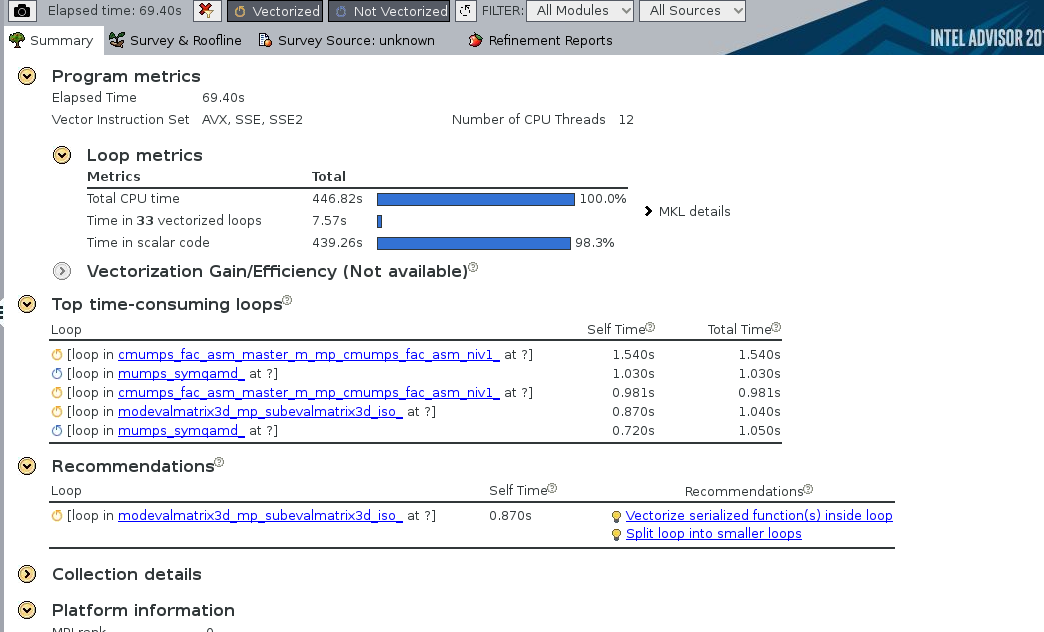
\includegraphics[height=13cm,width=15cm]{images/advisor.png}
    \caption{Intel$^{\mbox{\scriptsize{\textregistered}}}$ Advisor: Collect survey}
\label{advisor} 
\end{figure} 
\item \textbf{Intel$^{\mbox{\scriptsize{\textregistered}}}$ VTune Amplifier}
VTune Amplifier is a performance profiler from Intel$^{\mbox{\scriptsize{\textregistered}}}$. it can identify where in the code time is being spent in both serial and threaded applications. For threaded applications, it can also determine the amount of concurrency and identify bottlenecks created by synchronization primitives. Users can use graphic interface (GUI) to get deep analysis of hotspots and bottlenecks. The figure \ref{VTune} shows the user interface of VTune Amplifier.

\begin{figure}[!h]
\centering 
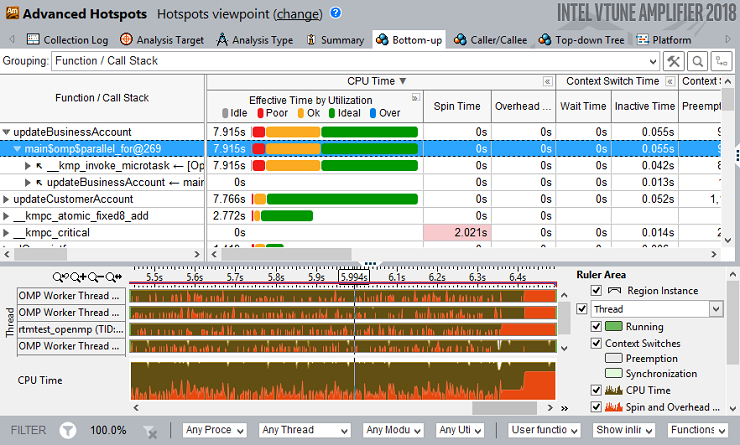
\includegraphics[height=13cm,width=15cm]{images/VTune.png}
    \caption{Intel$^{\mbox{\scriptsize{\textregistered}}}$ VTune Amplifier: Hotspot analysis}
\label{VTune} 
\end{figure} 
\item \textbf{Allinea Map :}
Allinea MAP is the profiler for parallel, multithreaded or single threaded C, C++, Fortran and F90 codes.  It provides in depth analysis and bottleneck pinpointing to the source line.  Unlike most profilers, it's designed to be able to profile pthreads, OpenMP or MPI for parallel and threaded code. It exposes a wide set of performance problems and bottlenecks by measuring:
\begin{itemize}
\item Computation - with self and child and call tree representations over time
\item Thread activity - to identify over-subscribed cores and sleeping threads that waste available CPU time for OpenMP and pthreads
\item Instruction types (for \verb|x86_64|) - to show use of vector-units or other performance extensions
\item Synchronization, communication and workload imbalance for MPI or multi-process usage
\item I/O performance and time spent in I/O - to identify bottlenecks in shared or local file systems
\end{itemize}
The figure \ref{allinea} shows an example of analysis of selected region. 

\begin{figure}[!h]
\centering 
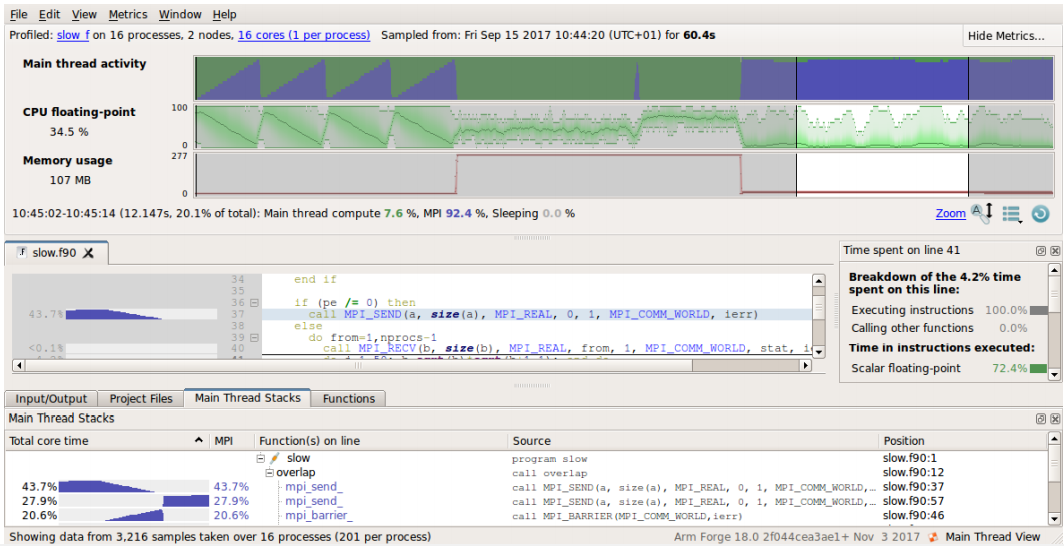
\includegraphics[height=13cm,width=15cm]{images/allinea.png}
    \caption{Allinea map:Map with a region of time selected}
\label{VTune} 
\end{figure} 
 
\item \textbf{BPM (MPIPROF) :}
BPM Profiler developed by Bull Atos group is is a library to extract MPI information like Statistic per process,communication matrix and timeline.
\item \textbf{Bull IO Instrumentation} (Note available)
\end{itemize}
\subsection{Optimization Libraries}
There exists many software using by HPC developers to optimize Math calculus, Memory consumption, communication, IA algorithms and so on : \textit{Math Kernel Library} (\textbf{MKL}) from Intel, \textit{Basic Linear Algebra Subprograms} (\textbf{BLAS}), \textit{Linear Algebra PACKage} (\textbf{LAPACK}) and \textbf{ScaLAPACK}, \textit{Portable, Extensible Toolkit for Scientific Computation} (\textbf{PETSc}), \textit{Hierarchical Data Format 5} (\textbf{HDF5}), \textit{Intel}$^{\mbox{\scriptsize{\textregistered}}}$ \textit{Data Analytics Acceleration Library} (\textbf{Intel}$^{\mbox{\scriptsize{\textregistered}}}$ \textbf{DAAL}) etc.

